\documentclass[tikz,border=4pt]{standalone}
\usepackage{libertine}
\usetikzlibrary{arrows.meta,calc,positioning,fit,backgrounds,shapes.geometric}
\definecolor{paperink}{HTML}{263441}
\definecolor{papermuted}{HTML}{647481}
\definecolor{paperline}{HTML}{CCD5DB}
\definecolor{paperblue}{HTML}{2D5F91}
\definecolor{paperbluefill}{HTML}{EFF5FA}
\definecolor{paperorange}{HTML}{B66731}
\definecolor{paperorangefill}{HTML}{FCF4EB}
\definecolor{papergreen}{HTML}{3F7558}
\definecolor{papergreenfill}{HTML}{EFF6F1}
\tikzset{
  papertext/.style={font=\footnotesize, text=paperink},
  papermini/.style={font=\scriptsize, text=papermuted},
  paneltitle/.style={font=\footnotesize\bfseries, text=paperink},
  bluebox/.style={draw=paperblue, fill=paperbluefill, rounded corners=1pt,
    line width=.6pt, font=\footnotesize, text=paperink, align=center,
    inner xsep=6pt, inner ysep=5pt},
  orangebox/.style={draw=paperorange, fill=paperorangefill, rounded corners=1pt,
    line width=.6pt, font=\footnotesize, text=paperink, align=center,
    inner xsep=6pt, inner ysep=5pt},
  greenbox/.style={draw=papergreen, fill=papergreenfill, rounded corners=1pt,
    line width=.6pt, font=\footnotesize, text=paperink, align=center,
    inner xsep=6pt, inner ysep=5pt},
  graybox/.style={draw=paperline, fill=white, rounded corners=1pt,
    line width=.6pt, font=\footnotesize, text=paperink, align=center,
    inner xsep=6pt, inner ysep=5pt},
  orangeflow/.style={-{Stealth[length=2mm]}, draw=paperorange, line width=1pt},
  blueflow/.style={-{Stealth[length=2mm]}, draw=paperblue, line width=1.15pt},
  greenflow/.style={-{Stealth[length=2mm]}, draw=papergreen, line width=1pt},
  grayflow/.style={-{Stealth[length=1.8mm]}, draw=papermuted, line width=.65pt}
}

\begin{document}
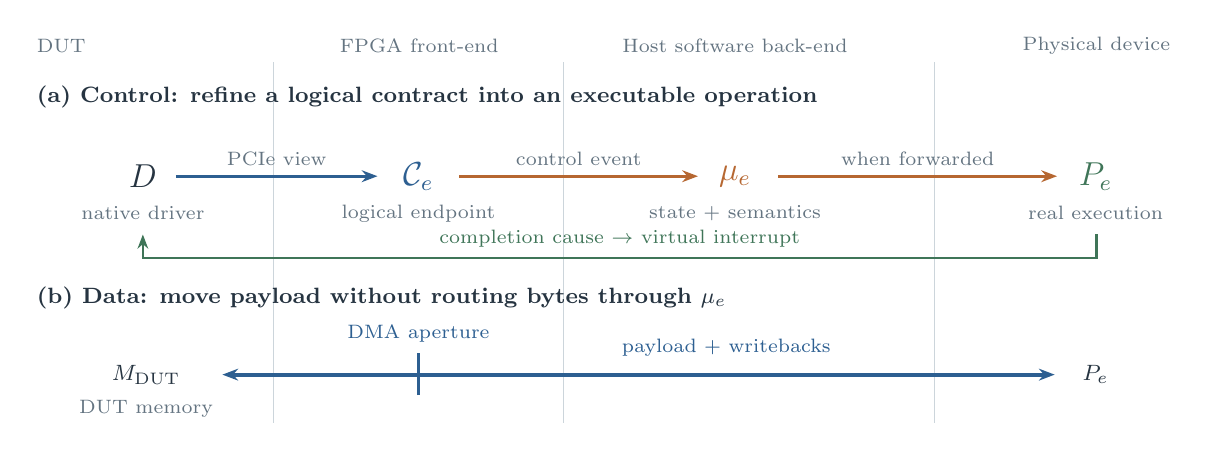
\begin{tikzpicture}[x=1cm,y=1cm]
  % A contract-to-execution view, not a physical wiring diagram.
  \node[papermini, anchor=west] at (.15,5.17) {DUT};
  \node[papermini] at (5.13,5.17) {FPGA front-end};
  \node[papermini] at (9.14,5.17) {Host software back-end};
  \node[papermini] at (13.73,5.17) {Physical device};
  \draw[paperline] (3.28,4.96) -- (3.28,.38);
  \draw[paperline] (6.96,4.96) -- (6.96,.38);
  \draw[paperline] (11.67,4.96) -- (11.67,.38);

  \node[paneltitle, anchor=west] at (.15,4.52) {(a) Control: refine a logical contract into an executable operation};
  \node[font=\large, text=paperink] (drv) at (1.62,3.51) {$D$};
  \node[papermini] at (1.62,3.04) {native driver};
  \node[font=\large, text=paperblue] (con) at (5.12,3.51) {$\mathcal{C}_e$};
  \node[papermini] at (5.12,3.04) {logical endpoint};
  \node[font=\large, text=paperorange] (med) at (9.14,3.51) {$\mu_e$};
  \node[papermini] at (9.14,3.04) {state + semantics};
  \node[font=\large, text=papergreen] (phy) at (13.72,3.51) {$P_e$};
  \node[papermini] at (13.72,3.04) {real execution};
  \draw[blueflow] (2.04,3.51) -- node[papermini, above] {PCIe view} (4.60,3.51);
  \draw[orangeflow] (5.64,3.51) -- node[papermini, above] {control event} (8.67,3.51);
  \draw[orangeflow] (9.69,3.51) -- node[papermini, above] {when forwarded} (13.23,3.51);
  \draw[papergreen, line width=.85pt, -{Stealth[length=1.8mm]}]
    (13.73,2.77) -- (13.73,2.47) -- node[papermini, above, text=papergreen]
    {completion cause $\to$ virtual interrupt} (1.62,2.47) -- (1.62,2.77);

  \node[paneltitle, anchor=west] at (.15,1.96) {(b) Data: move payload without routing bytes through $\mu_e$};
  \node[papertext] at (1.66,.99) {$M_{\mathrm{DUT}}$};
  \node[papermini] at (1.66,.56) {DUT memory};
  \node[papertext] at (13.72,.99) {$P_e$};
  \draw[paperblue, line width=1.35pt, {Stealth[length=2mm]}-{Stealth[length=2mm]}]
    (2.63,.99) -- (13.20,.99);
  \draw[paperblue, line width=1pt] (5.12,.73) -- (5.12,1.26);
  \node[papermini, above, text=paperblue] at (5.12,1.28) {DMA aperture};
  \node[papermini, above, text=paperblue] at (9.03,1.10) {payload + writebacks};
\end{tikzpicture}
\end{document}
